\chapter{Descripción del trabajo} \label{cap:descripcionTrabajo}

En este capítulo se describe el editor de mallas desarrollado para este trabajo. En primer lugar, se presenta a grandes rasgos la arquitectura general del programa. A continuación, se enumeran las distintas funcionalidades que ofrece, y por último se detalla cómo se ha implementado cada una de ellas.

\section{Estructura del programa}

El flujo de la aplicación para la edición de una malla es el siguiente: el modelo se carga desde un archivo en disco, y se transforma en una representación interna para su edición. Sobre esta representación, el usuario aplica una serie de operaciones de selección y transformación, que quedan representados en la visualización del modelo. Finalmente, la malla se puede exportar a un nuevo archivo en disco. La figura~\ref{fig:estructura-programa} ilustra este flujo, así como las dos partes principales en las que se organiza la aplicación para llevarlo a cabo.

\subsection{Interfaz de usuario} \label{sec:UI}

La ventana principal de la aplicación se organiza en torno a tres elementos: un lienzo central, donde se renderiza y edita la escena tridimensional, una barra de herramientas, desde la que el usuario controla el modo de edición activo en cada momento, y desde la cual puede cargar y guardar la malla trabajada, y desplegar un panel con información adicional sobre el control de la cámara, y un panel de transformación, que muestra y permite modificar la posición en la escena del elemento actualmente seleccionado.

El lienzo ocupa la mayor parte del área central de la ventana, y constituye la superficie sobre la que se dibuja la malla y se capturan las interacciones del usuario. La barra de herramientas, en la zona superior de la ventana, agrupa las distintas acciones disponibles en botones organizados por categorías, cada una representada mediante un conjunto de botones mutuamente excluyentes: el modo de selección (vértices, aristas o polígonos), el modo de transformación (traslación, rotación o escalado), el eje sobre el que se restringe dicha transformación, el modo de renderizado (sólido o \textit{wireframe}) y el tipo de proyección de la cámara (perspectiva u ortogonal). El panel lateral, en el lateral derecho de la ventana, permite además ajustar numéricamente la posición de la selección actual mediante tres campos correspondientes a sus coordenadas X, Y y Z.

La interfaz de usuario se implementa mediante Qt, una biblioteca externa diseñada para el desarrollo de interfaces gráficas, encargada de construir la ventana principal y todos sus elementos (lienzo, barra de herramientas y panel lateral), así como de gestionar el menú de importación y exportación de modelos (sección~\ref{sec:UI}).

Cada acción de la barra de herramientas se conecta directamente, mediante el sistema de señales de Qt, a un método de la lógica de edición que modifica su estado. Esta vía de comunicación es independiente del resto del input de la aplicación: mientras que el movimiento del ratón sobre el lienzo o la mayoría de las teclas del teclado se centralizan y consultan explícitamente en cada iteración del bucle principal (sección~\ref{sec:input}), las acciones de la barra de herramientas tienen efecto de forma inmediata en el momento en que se pulsan, ya sea con el ratón o mediante su atajo de teclado asociado.

\subsection{Lógica del programa}

La lógica del programa es responsable de mantener y modificar el estado de la malla que se está editando, y queda coordinada por la clase \texttt{Editor}, que integra las siguientes responsabilidades:

\begin{itemize}
    \item La malla en sí, representada por la clase \texttt{Mesh}, que almacena su geometría y ofrece además las operaciones de carga y guardado del modelo desde y hacia archivo (sección~\ref{sec:mesh}).
    \item La selección de elementos de la malla, implementada por la clase \texttt{Selector} (sección~\ref{sec:seleccion}).
    \item Las operaciones de edición aplicadas sobre los elementos seleccionados, definidas en la clase \texttt{MeshManipulator} (sección~\ref{sec:edicion}).
    \item La cámara, gestionada por la clase \texttt{Camera}, que determina desde qué posición y con qué proyección se observa la escena (sección~\ref{sec:camera}).
    \item El renderizado del modelo y de los elementos seleccionados, cuya responsabilidad no recae en una única clase, sino que se reparte entre \texttt{Mesh} (que dibuja su propia geometría), los programas de shaders (sección~\ref{sec:shaders}) y \texttt{Camera} (sección~\ref{sec:camera}), que aporta las matrices de vista y proyección necesarias. Es el propio \texttt{Editor} quien coordina este proceso en cada frame, combinando dichas matrices con la matriz de modelo y emitiendo las llamadas de dibujado correspondientes.
\end{itemize}

Cabe destacar que la separación entre la interfaz y la lógica del programa no es absoluta: por conveniencia, el propio \texttt{Editor} hace uso del sistema de señales de Qt para comunicar a la interfaz cambios en la posición del elemento actualmente seleccionado, y además comunica a la lógica cambios en los valores de la interfaz, de manera que la modificación de alguno de los dos afecta al otro.

\begin{figure}[htbp]
    \centering
    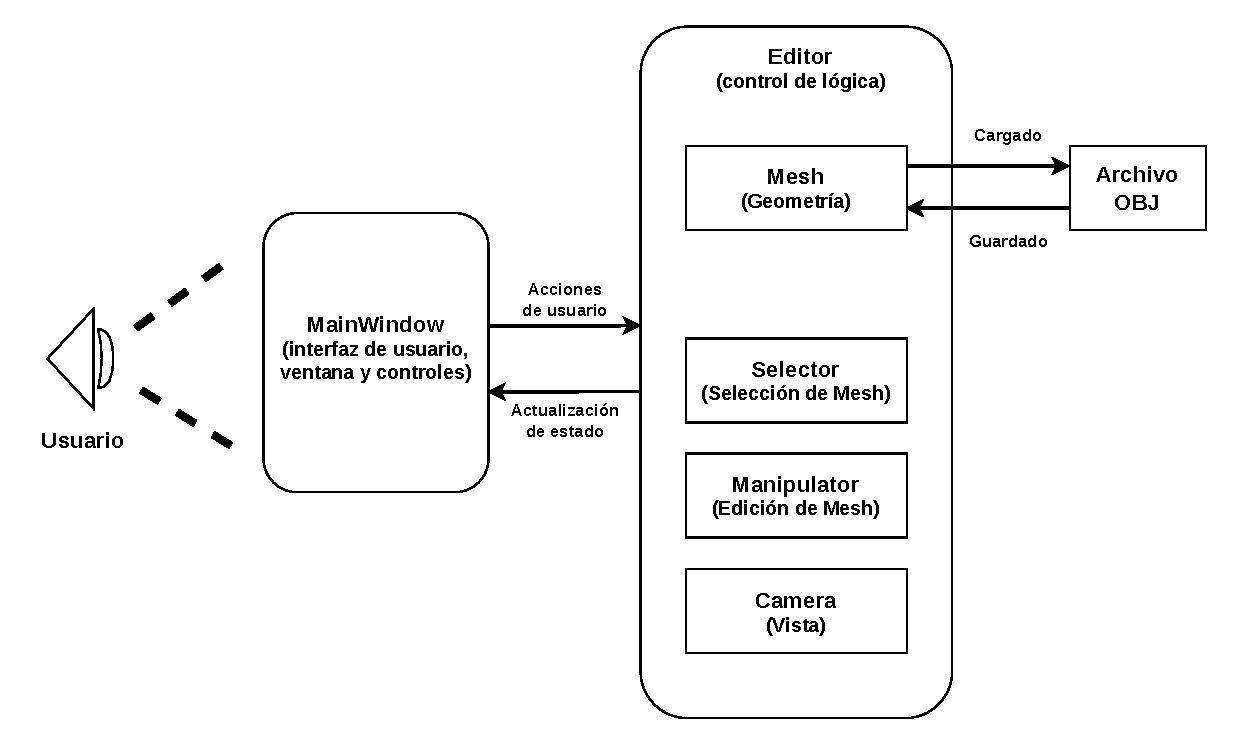
\includegraphics[width = 1.0\textwidth]{TFGTeXiS-UTF8/Imagenes/Vectorial/EstructuraPrograma.drawio.pdf}
    \caption{Estructura del programa.}
    \label{fig:estructura-programa}
\end{figure}

\section{Funcionalidades}

En esta sección se describen las funcionalidades que ofrece el editor desde la perspectiva del usuario, sin entrar en detalles de su implementación, los cuales se tratan en la sección~\ref{sec:detalles-implementacion}.

\subsection{Importación y exportación de modelos}

El editor permite cargar modelos tridimensionales en formato OBJ desde el menú \emph{Archivo > Abrir}, así como guardar el estado actual de la malla editada en el mismo formato mediante \emph{Archivo > Guardar} (figura~\ref{fig:UI}).

\begin{figure}[htbp]
    \centering
    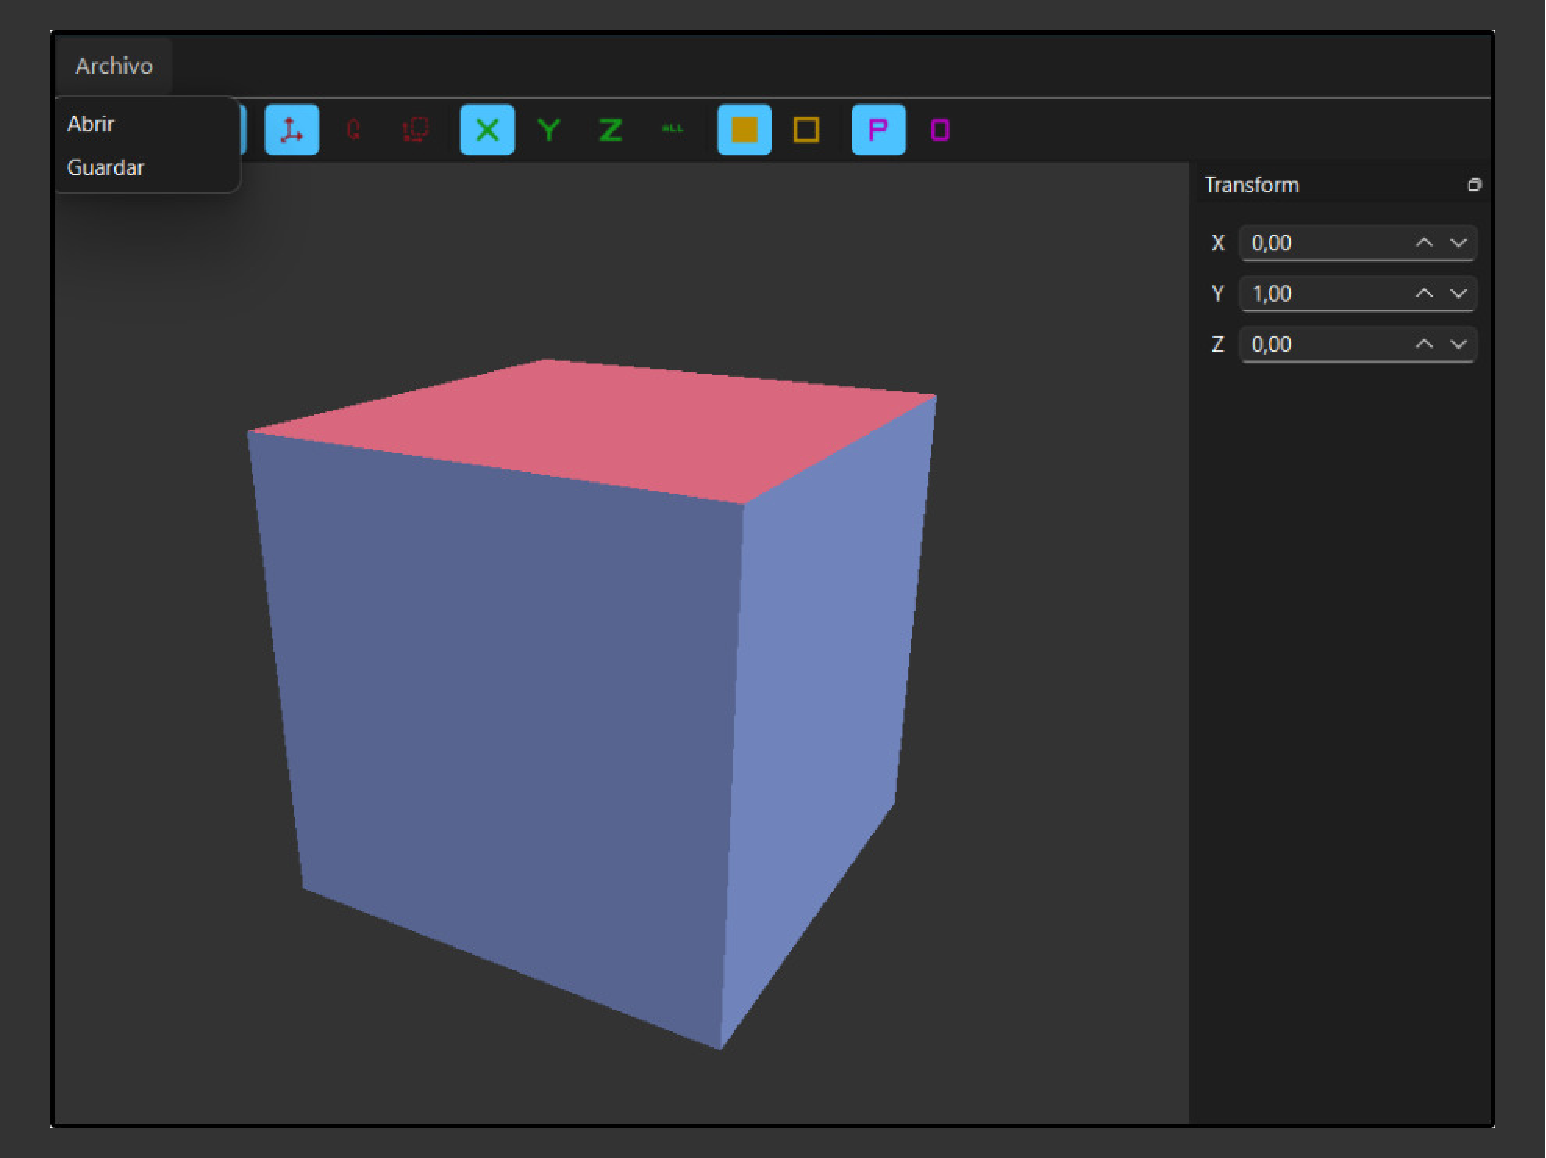
\includegraphics[width=1\textwidth]{TFGTeXiS-UTF8/Imagenes/Vectorial/Funcionalidades/UI.pdf}
    \caption{Interfaz de usuario de la aplicación.}
    \label{fig:UI}
\end{figure}

\subsection{Visualización de la escena}

El usuario puede observar el modelo desde cualquier ángulo mediante el control de la cámara: manteniendo pulsado el botón central del ratón se orbita alrededor del modelo, combinándolo con la tecla \texttt{Shift} se desplaza la vista lateralmente (paneo), y mediante la rueda del ratón se acerca o aleja la cámara (zoom). Adicionalmente, la tecla \texttt{F} recentra la cámara sobre el modelo (figura~\ref{fig:controles-camara}).

\begin{figure}[htbp]
    \centering
    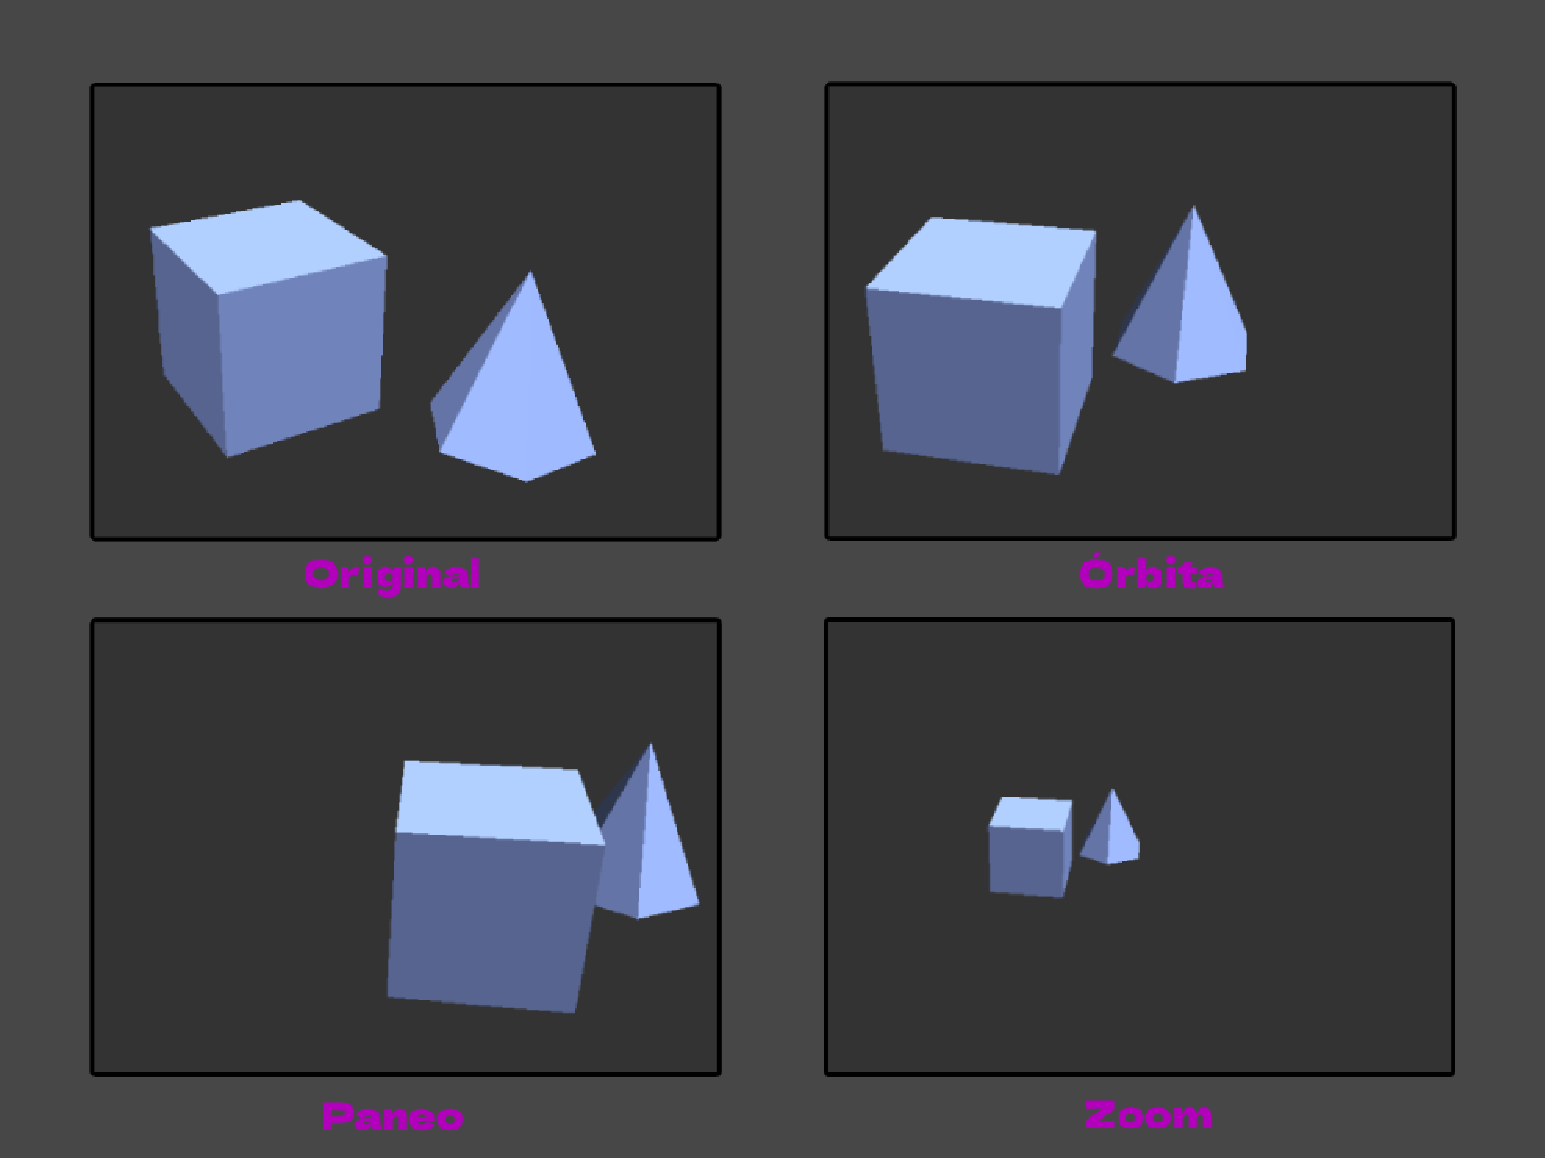
\includegraphics[width=0.8\textwidth]{TFGTeXiS-UTF8/Imagenes/Vectorial/Funcionalidades/Camara.pdf}
    \caption{Controles de la cámara.}
    \label{fig:controles-camara}
\end{figure}

El editor ofrece dos tipos de proyección, seleccionables desde la barra de herramientas: perspectiva, en la que los objetos más alejados de la cámara aparecen de menor tamaño, y ortogonal, en la que dicho efecto no se produce.

Asimismo, el modelo puede visualizarse en modo sólido, con su superficie completamente rellena, o en modo \emph{wireframe}, mostrando únicamente las aristas de la malla (figura~\ref{fig:perspectiva-ortogonal}). 

\begin{figure}[htbp]
    \centering
    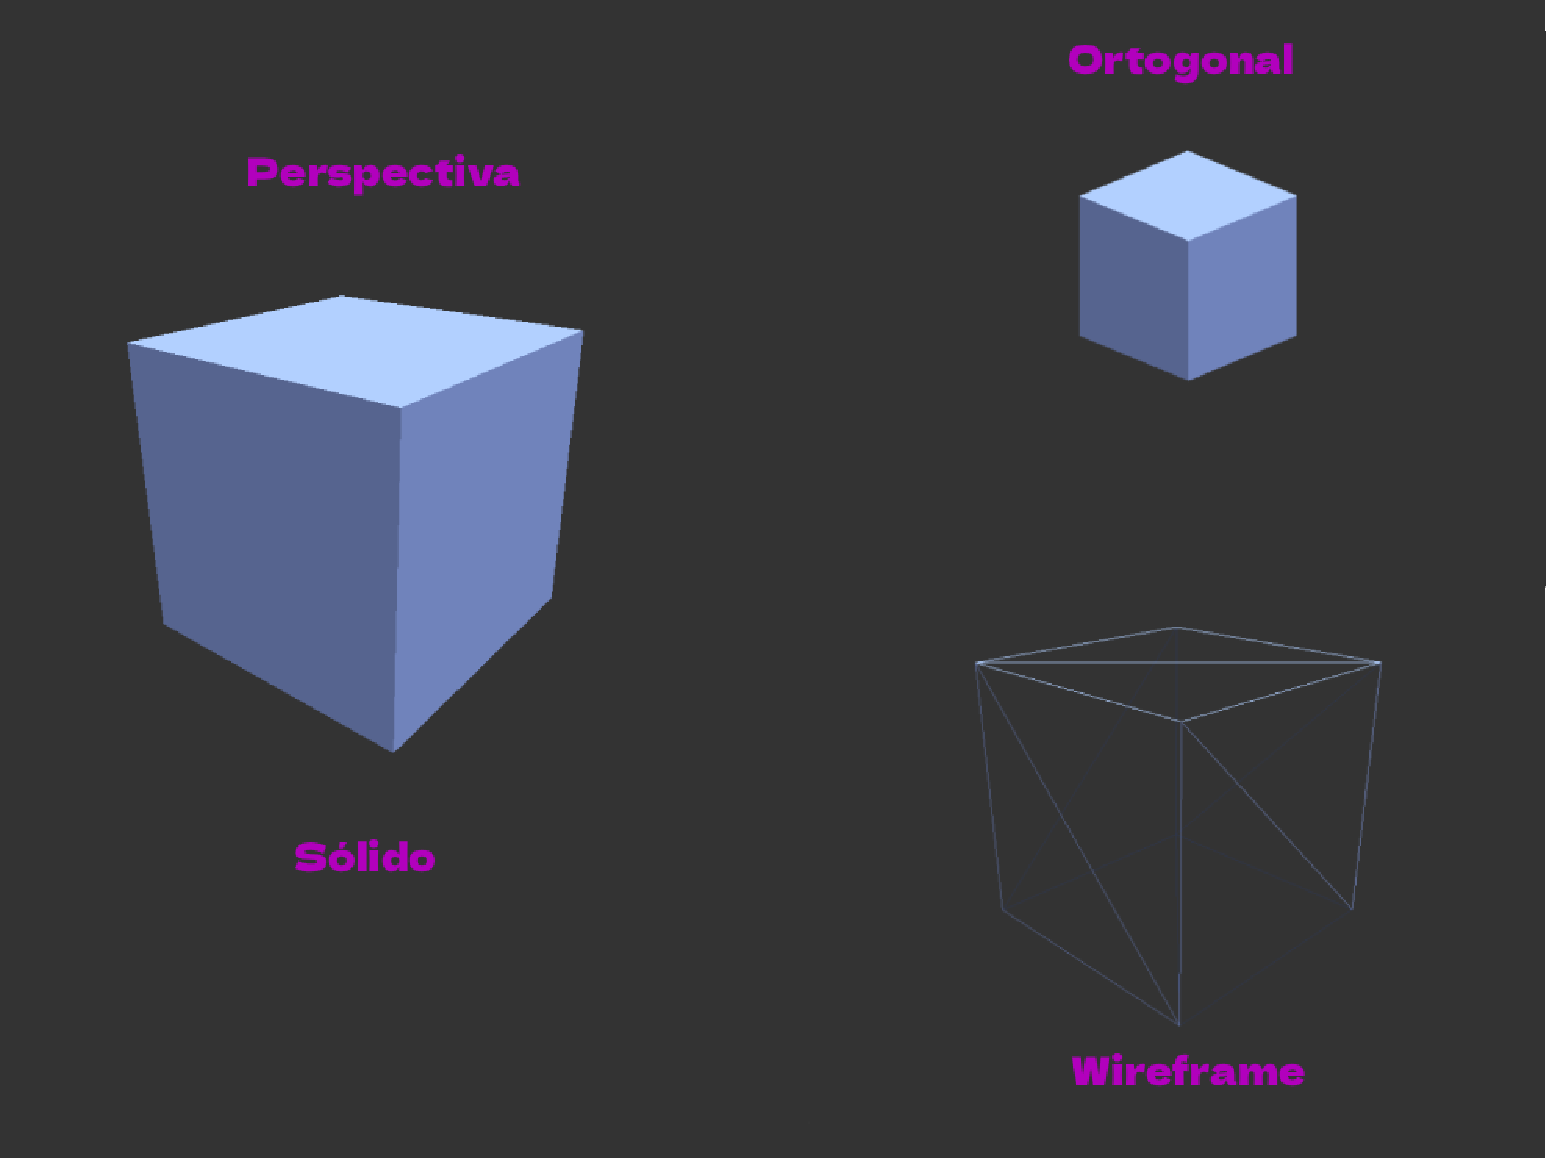
\includegraphics[width=0.8\textwidth]{TFGTeXiS-UTF8/Imagenes/Vectorial/Funcionalidades/Ortogonal_Wireframe.pdf}
    \caption{Comparación entre proyección perspectiva/ortogonal, y renderizado sólido/wireframe.}
    \label{fig:perspectiva-ortogonal}
\end{figure}

\subsection{Selección de elementos}

El usuario puede seleccionar tres tipos de elementos de la malla: vértices, aristas o polígonos, alternando entre ellos desde la barra de herramientas. Al hacer clic izquierdo sobre un elemento, este queda seleccionado; manteniendo pulsada la tecla \texttt{Shift} durante el clic, la selección se añade a la ya existente en lugar de sustituirla, permitiendo seleccionar varios elementos a la vez (figura~\ref{fig:seleccion}).

\begin{figure}[htbp]
    \centering
    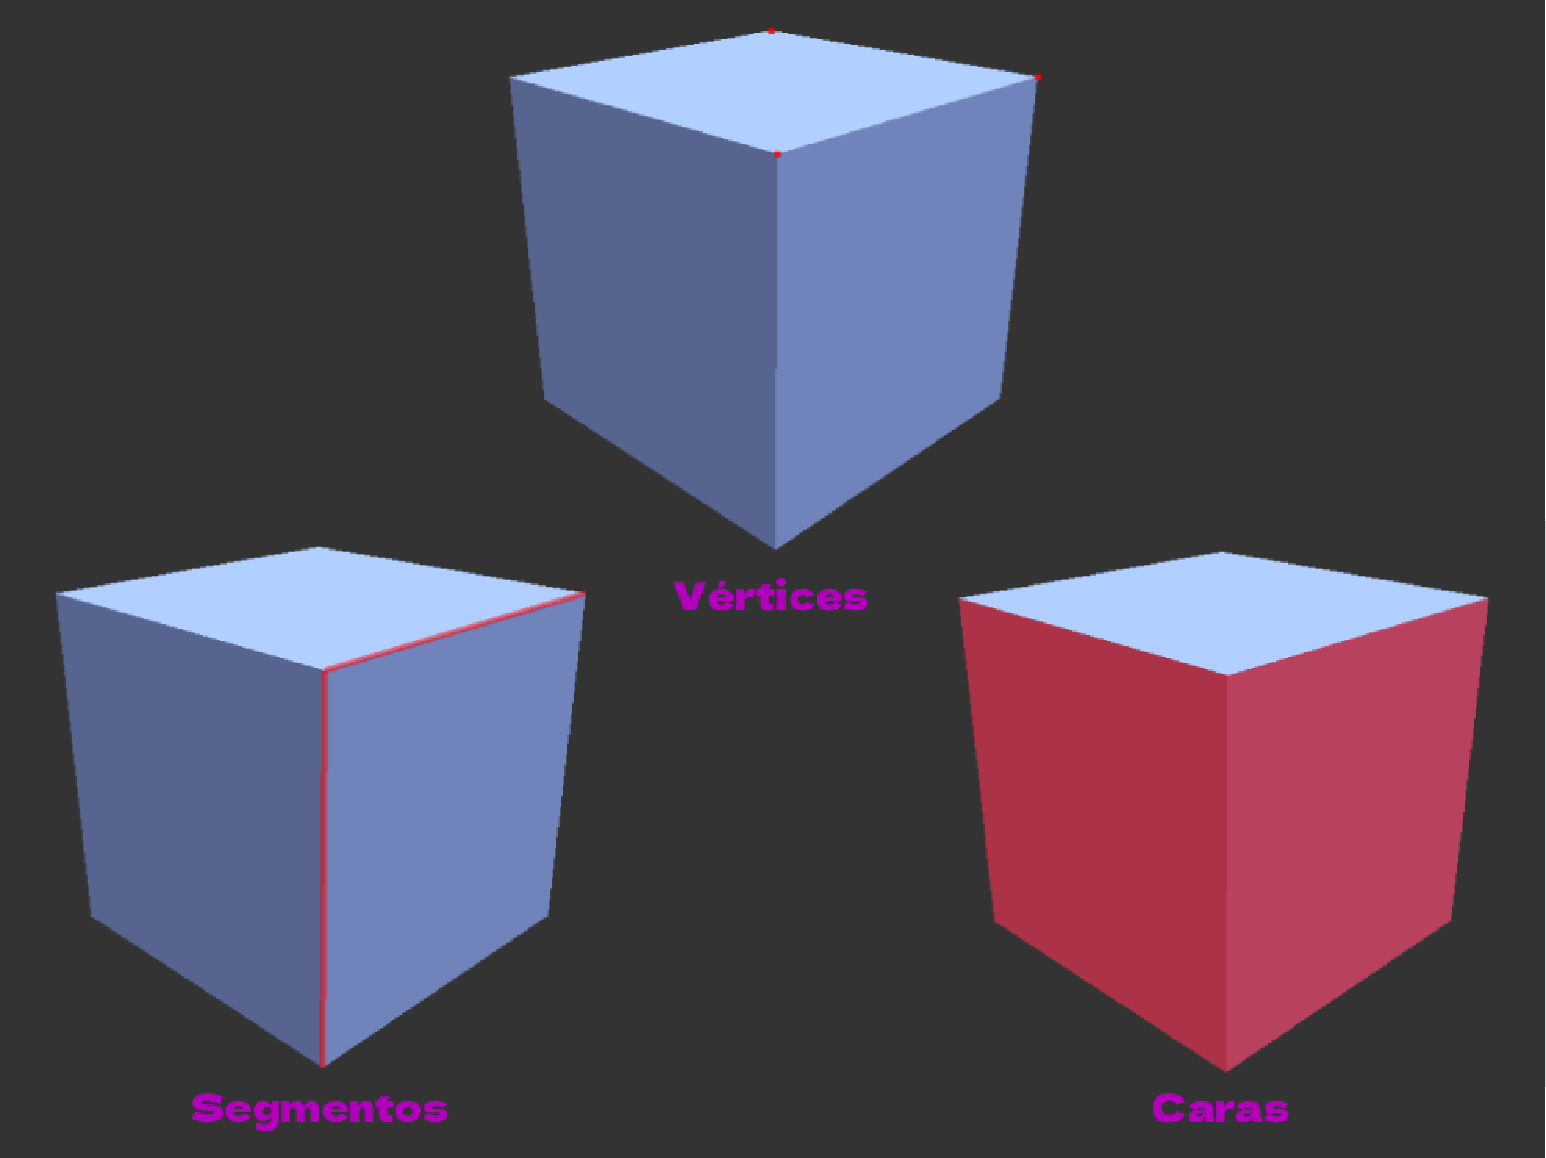
\includegraphics[width=0.8\textwidth]{TFGTeXiS-UTF8/Imagenes/Vectorial/Funcionalidades/Selecciones.pdf}
    \caption{Selección de vértices, segmentos y polígonos}
    \label{fig:seleccion}
\end{figure}

\subsection{Edición de la malla} \label{sec:edicion}

Sobre los elementos seleccionados pueden aplicarse las siguientes operaciones:

\begin{itemize}
    \item \textbf{Transformación}: traslación, rotación o escalado de la selección, arrastrando el ratón tras elegir el modo correspondiente en la barra de herramientas. La transformación puede restringirse a un único eje (X, Y o Z) o aplicarse libremente sobre los tres a la vez. Adicionalmente, la posición del elemento seleccionados (o posición media, en el caso de mútiples elementos) puede ajustarse numéricamente desde un panel lateral de la interfaz (figura~\ref{fig:UI}) (figura~\ref{fig:transformaciones}).

    \begin{figure}[htbp]
        \centering
        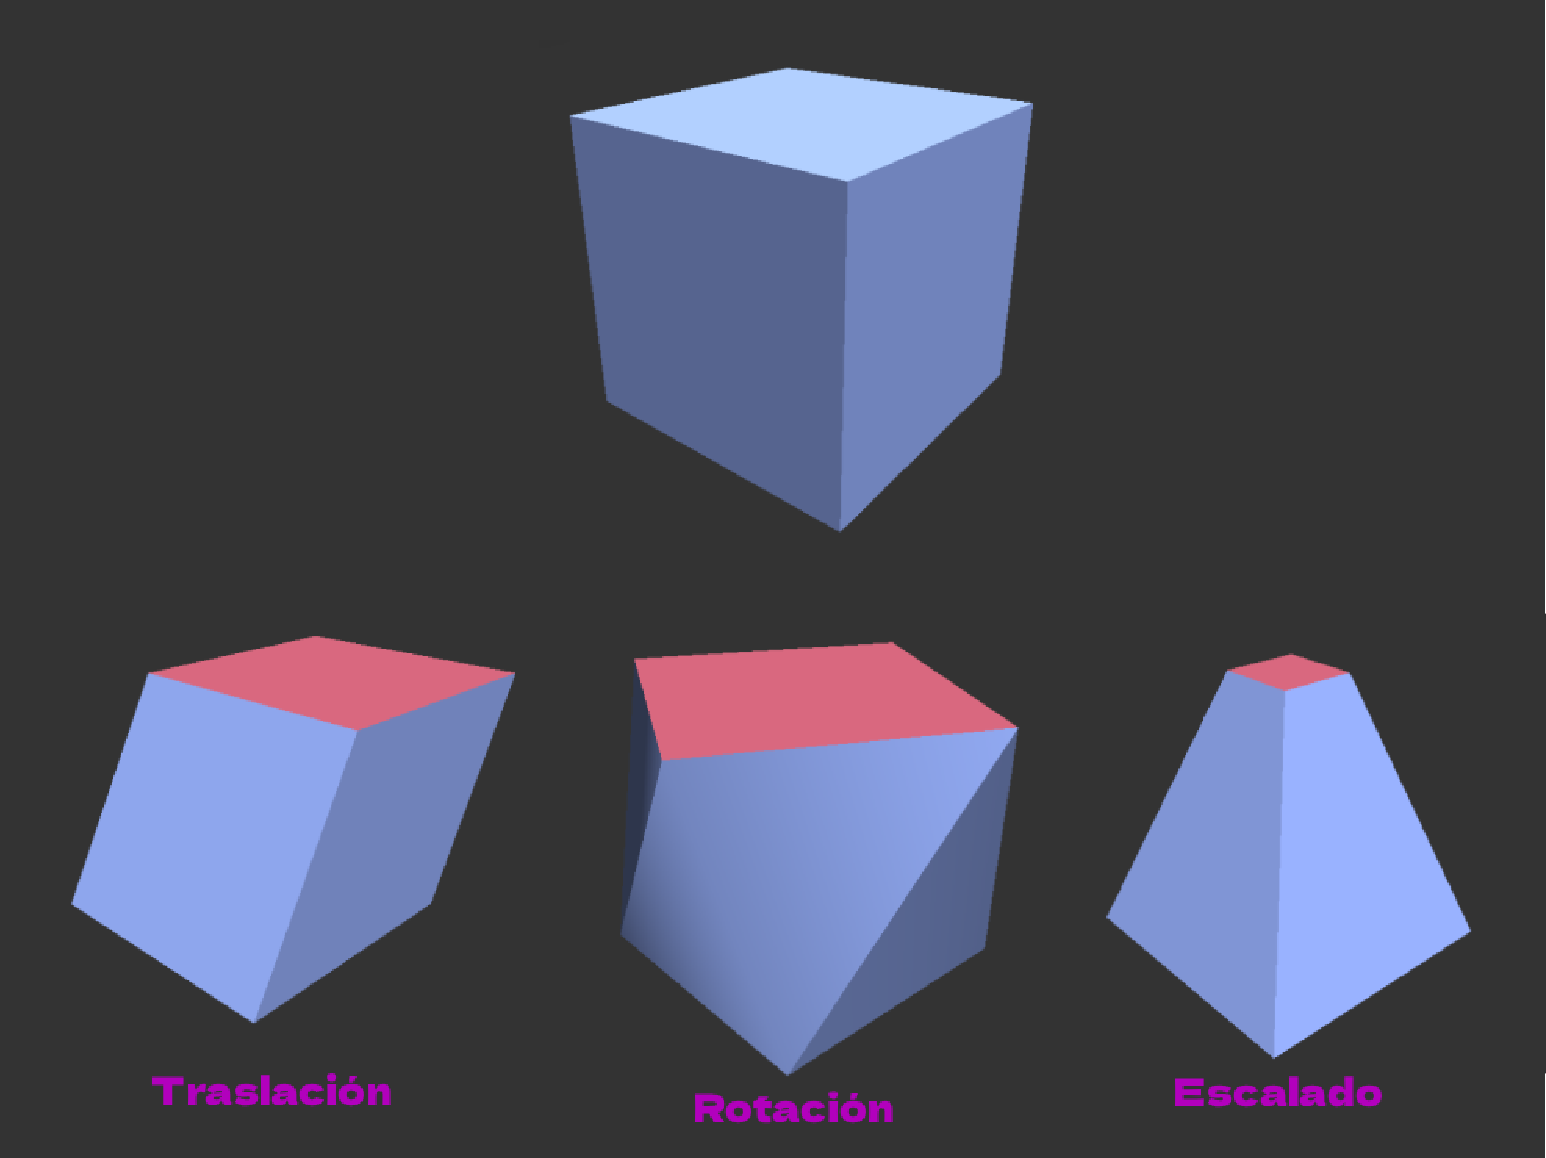
\includegraphics[width=0.8\textwidth]{TFGTeXiS-UTF8/Imagenes/Vectorial/Funcionalidades/Transformaciones.pdf}
        \caption{Tipos de transformaciones}
        \label{fig:transformaciones}
    \end{figure}

    \item \textbf{Eliminación}: borra los elementos actualmente seleccionados de la malla (figura~\ref{fig:extrusion_eliminacion}).

    \item \textbf{Extrusión}: genera nueva geometría a partir de los polígonos seleccionados, desplazándolos en la dirección de su normal y conectando los bordes resultantes con la superficie original (figura~\ref{fig:extrusion_eliminacion}).

    \begin{figure}[htbp]
        \centering
        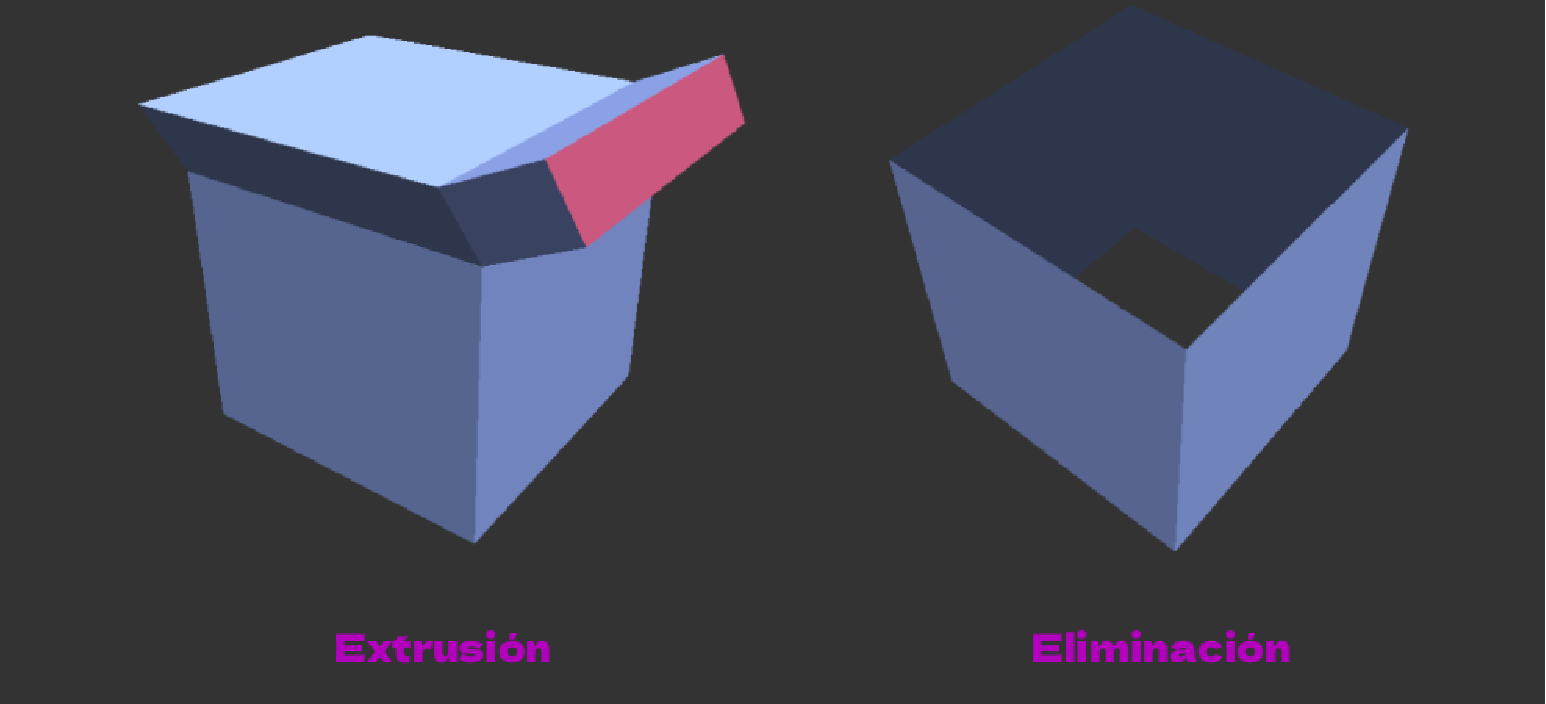
\includegraphics[width=0.8\textwidth]{TFGTeXiS-UTF8/Imagenes/Vectorial/Funcionalidades/Extrusion_Eliminacion.pdf}
        \caption{Extrusión y eliminacion de caras seleccionadas.}
        \label{fig:extrusion_eliminacion}
    \end{figure}
\end{itemize}

Durante todo el proceso de edición, los elementos actualmente seleccionados se resaltan visualmente sobre la malla, permitiendo al usuario identificar en todo momento sobre qué está operando.

\subsection{Atajos de teclado}

La tabla~\ref{tab:atajos} resume los atajos de teclado disponibles en el editor.

\begin{table}[htbp]
\centering
\begin{tabular}{ll}
\hline
\textbf{Tecla} & \textbf{Acción} \\
\hline
1 / 2 / 3 & Seleccionar vértices / aristas / polígonos \\
G / R / S & Modo de transformación: mover / rotar / escalar \\
X / Y / Z / A & Restringir transformación al eje X / Y / Z / todos \\
Q / W & Modo de renderizado: sólido / wireframe \\
P / O & Proyección: perspectiva / ortogonal \\
E & Extruir la selección poligonal \\
Supr & Eliminar la selección \\
Clic & Selección / deselección \\
Shift (+ clic) & Selección aditiva \\
F & Recentrar la cámara \\
Botón central + arrastre & Orbitar la cámara \\
Shift + botón central + arrastre & Desplazar la cámara (paneo) \\
Rueda del ratón & Acercar / alejar la cámara (zoom) \\
\hline
\end{tabular}
\caption{Atajos de teclado del editor.}
\label{tab:atajos}
\end{table}

\section{Detalles de implementación} \label{sec:detalles-implementacion}

A continuación se detalla el funcionamiento de los distintos componentes y sistemas del programa.

\subsection{Sistema de renderizado}

El primer requisito del editor consiste en disponer de un sistema capaz de representar modelos tridimensionales.

\subsubsection{Creación de ventana y contexto con Qt}

La biblioteca seleccionada para la creación de la ventana y el contexto de la aplicación fue Qt. Dentro de Qt se define un \texttt{QOpenGLWidget} \texttt{Canvas}, que gestiona el bucle principal de la aplicación a través del método \texttt{paintGL}. Este \texttt{Canvas} contiene al \texttt{Editor}, responsable de la lógica del programa, cuyo bucle principal es invocado desde el propio \texttt{Canvas} en cada frame.

Para poder invocar las funciones de OpenGL desde \texttt{Canvas}, es necesario obtener el contexto de OpenGL en tiempo de ejecución. Para ello, se recurre a (\texttt{QOpenGLContext::\allowbreak currentContext()}), a partir del cual se obtienen las direcciones de las funciones de OpenGL necesarias.

\subsubsection{Shaders} \label{sec:shaders}

Los shaders se almacenan en archivos independientes y se cargan durante la inicialización del sistema de renderizado.  Estos programas están implementados en GLSL, el lenguaje de shaders de OpenGL, orientado a programas gráficos y que proporciona operaciones específicas entre vectores y matrices \cite{learnOpenGL_shaders, learnopengl_book}.

La aplicación utiliza dos programas de shaders: uno de \textit{iluminación}, empleado para representar la superficie de la malla, y uno de \textit{selección}, utilizado para resaltar visualmente los elementos seleccionados por el usuario durante la edición. Cada programa está compuesto por un shader de vértices y un shader de fragmentos.

\paragraph{Shader de iluminación:} \label{p:shader_iluminacion}El shader de vértices (mostrado en \ref{lst:shader_vertices_iluminacion}) recibe como atributos de entrada la posición y la normal de cada vértice. A partir de estos, calcula la posición del vértice en coordenadas de mundo, multiplicando su posición local por la matriz de modelo, y transforma su normal mediante la matriz normal (la traspuesta de la inversa de la matriz de modelo), necesaria para que la normal se transforme correctamente incluso en presencia de escalados no uniformes de la malla. Ambos valores se envían como variables de salida, que el rasterizador interpola automáticamente para cada fragmento situado dentro del triángulo antes de llegar al shader de fragmentos.

\begin{listing}[htb]
\begin{minted}[breaklines, fontsize=\small]{glsl}
layout (location = 0) in vec3 aPos;
layout (location = 1) in vec3 aNormal;

uniform mat4 MVP;
uniform mat4 model;
uniform mat3 normalMatrix;

out vec3 FragPos;
out vec3 Normal;

void main()
{
    FragPos = vec3(model * vec4(aPos, 1.0));
    Normal = normalMatrix * aNormal;

    gl_Position = MVP * vec4(aPos, 1.0);
}
\end{minted}
\caption{Shader de vértices del programa de iluminación.}
\label{lst:shader_vertices_iluminacion}
\end{listing}

El shader de fragmentos (listing~\ref{lst:shader_fragmentos_iluminacion}) calcula la iluminación de cada fragmento a partir de la normal interpolada y de una única fuente de luz direccional. La dirección de dicha luz se recibe mediante el uniform \texttt{lightDir}, cuyo valor se fija directamente desde el código de la aplicación como un vector constante, sin que el usuario pueda modificarlo desde la interfaz.

El modelo de iluminación empleado puede entenderse como una instancia particular del modelo de Phong en la que el término especular es nula, quedando únicamente los términos ambiente y difuso. El término ambiente es una constante fija, y el término difuso se calcula según la ley de Lambert, esto es, el producto escalar entre la normal de la superficie y la dirección hacia la luz, limitado a valores no negativos para evitar iluminar caras opuestas a la fuente. El resultado se aplica directamente sobre el color base del objeto (\texttt{objectColor}). Al no definirse un color independiente para la luz, esta se comporta como una fuente de luz blanca.

Cabe destacar que, al calcularse la iluminación por fragmento a partir de la normal interpolada en lugar de en el vértice, como ocurre en \emph{Gouraud shading}, la técnica empleada se corresponde con lo que se conoce como \emph{Phong shading}. Este término no debe confundirse con el modelo de iluminación de Phong: el primero es una técnica de interpolación, mientras que el segundo es el modelo de iluminación en sí (ambiente, difusa y especular), del cual, en este caso, se emplea la variante con componente especular nulo.

\begin{listing}[htb]
\begin{minted}[breaklines, fontsize=\small]{glsl}
out vec4 FragColor;

in vec3 FragPos;
in vec3 Normal;

uniform vec3 lightDir;
uniform vec3 objectColor;

void main()
{
    vec3 norm = normalize(Normal);
    vec3 light = normalize(-lightDir);

    float diff = max(dot(norm, light), 0.0);

    float ambient = 0.2;

    vec3 color = (ambient + diff) * objectColor;

    FragColor = vec4(color, 1.0);
}
\end{minted}
\caption{Shader de fragmentos del programa de iluminación.}
\label{lst:shader_fragmentos_iluminacion}
\end{listing}

\paragraph{Shader de selección:}

El shader de selección tiene como propósito resaltar visualmente los elementos de la malla que el usuario tiene actualmente seleccionados. A diferencia del shader de iluminación (párrafo~\ref{p:shader_iluminacion}), no recibe la normal de los vértices como atributo de entrada, únicamente su posición, ya que no necesita calcular ningún tipo de sombreado. En consecuencia, su shader de vértices (listing~\ref{lst:shader_vertices_seleccion}) se limita a transformar dicha posición.

\begin{listing}[htb]
\begin{minted}[breaklines, fontsize=\small]{glsl}
layout(location = 0) in vec3 vp;

uniform mat4 MVP;

void main()
{
    gl_Position = MVP * vec4(vp, 1.0);
}
\end{minted}
\caption{Shader de vértices del programa de selección.}
\label{lst:shader_vertices_seleccion}
\end{listing}

El shader de fragmentos asigna directamente un color rojo semitransparente a cada fragmento, sin depender de ninguna variable de entrada (listing~\ref{lst:shader_fragmentos_seleccion}).

\begin{listing}[htb]
\begin{minted}[breaklines, fontsize=\small]{glsl}
out vec4 FragColor;

void main()
{
    FragColor = vec4(1.0, 0.0, 0.0, 0.5);
}
\end{minted}
\caption{Shader de fragmentos del programa de selección.}
\label{lst:shader_fragmentos_seleccion}
\end{listing}

La selección se resuelve previamente en la CPU: la clase \texttt{Selector} mantiene los índices de los vértices, aristas o polígonos actualmente seleccionados, a partir de los cuales se construye, en cada frame, un vector con las posiciones de todos los vértices contenidos en estos elementos. Para los polígonos, dado que pueden tener más de tres vértices, se recurre a la misma triangulación en abanico empleada durante su selección (sección~\ref{sec:seleccion-poligonos}), añadiendo al vector los tres vértices de cada triángulo resultante.

Este vector se envía a la clase \texttt{SelectionRenderer}, que mantiene un único VAO y VBO compartido entre los tres tipos de elemento seleccionable. El \textit{buffer} se redimensiona en cada frame según el número de vértices a representar, mediante una llamada a \texttt{glBufferData}. Puesto que el modo de selección es excluyente entre vértices, aristas y polígonos, en un frame dado únicamente se dibuja un tipo de primitiva, lo que permite emitir toda la selección en una única llamada a \texttt{glDrawArrays}, con la primitiva de OpenGL correspondiente al tipo de elemento seleccionado (\texttt{GL\_POINTS}, \texttt{GL\_LINES} o \texttt{GL\_TRIANGLES}).

\subsubsection{Buffers} \label{sec:buffers}

Las mallas del editor mantienen su propio VBO, EBO y VAO, gestionados por la clase \texttt{Mesh}, asumiendo simultáneamente el papel de modelo de datos de la malla y el de propietaria de los recursos de OpenGL necesarios para su renderizado, sin que exista una separación entre una representación puramente lógica de la malla y una representación orientada a su visualización.

Los atributos de vértice se almacenan de forma entrelazada en un único VBO: cada elemento consecutivo del buffer es una estructura \texttt{Vertex} completa, que agrupa la posición y la normal de un mismo vértice de renderizado. De este modo, el contenido del buffer en memoria sigue el patrón \texttt{[posición$_0$, normal$_0$, posición$_1$, normal$_1$, \ldots]}.

Para que la GPU pueda interpretar correctamente este entrelazado, el VAO configura dos atributos sobre el mismo buffer, cada uno con un \emph{stride} igual al tamaño completo de la estructura \texttt{Vertex}, de modo que al leer un atributo la GPU sepa cuántos bytes debe avanzar para llegar al mismo atributo del siguiente vértice, saltando los datos intermedios que no le corresponden, y un \emph{offset} distinto para cada uno, que indica en qué posición dentro de dicha estructura comienza el atributo en cuestión: 0 para la posición, y el desplazamiento de \texttt{Normal} dentro de \texttt{Vertex} (obtenido mediante \texttt{offsetof}) para la normal (listing~\ref{lst:config_atrib_VAO}).

\begin{listing}[htb]
\begin{minted}[breaklines, fontsize=\small]{c++}
glVertexAttribPointer(0, 3, GL_FLOAT, GL_FALSE, sizeof(Vertex), nullptr);
glVertexAttribPointer(1, 3, GL_FLOAT, GL_FALSE, sizeof(Vertex), (void*)offsetof(Vertex, Normal));
\end{minted}
\caption{Configuración de atributos en el VAO.}
\label{lst:config_atrib_VAO}
\end{listing}

El EBO almacena los índices de cada polígono, de forma que la malla se renderiza como una malla indexada: los vértices compartidos entre varios triángulos de un mismo polígono se almacenan una única vez en el VBO y se referencian repetidamente desde el EBO.

Dado que la malla puede modificarse durante la edición, ambos buffers se crean con \texttt{GL\_DYNAMIC\_DRAW}, y se actualizan explícitamente cada vez que cambia la topología de la malla, volviendo a enviar su contenido completo a la GPU.

Cabe destacar que el resaltado visual de los elementos seleccionados (sección~\ref{shaders}) no reutiliza estos buffers: se renderiza mediante un componente independiente, encargado de generar y enviar a la GPU la geometría auxiliar correspondiente a los vértices, aristas o polígonos seleccionados en cada frame.

\subsection{Representación de la malla} \label{sec:mesh}

Para poder editar la malla mostrada en la ventana previamente creada, se define una representación interna de esta en el programa.

A pesar de aprovechar parcialmente la estructura de malla proporcionada por \texttt{tinyobjloader}, esta no ofrece dos elementos necesarios para la edición del modelo: una representación de las aristas de la malla, y una agrupación de los vértices que comparten una misma posición geométrica. Por este motivo se desarrolla una representación interna propia, descrita en los siguientes apartados.

Durante la carga del modelo es necesario transformar la representación proporcionada por \texttt{tinyobjloader} en esta representación interna. Este proceso resuelve dos necesidades distintas: por un lado, evitar la duplicación de vértices de renderizado idénticos, esto es, con la misma posición y la misma normal, y por otro, mantener agrupados aquellos vértices de renderizado que comparten una misma posición geométrica pero que, al pertenecer a caras con distinta orientación, poseen normales distintas y por tanto no pueden fusionarse en un único vértice de renderizado. El primer proceso reduce el número de vértices almacenados, mientras que el segundo no elimina ningún vértice, sino que mantiene una referencia entre aquellos que, aun siendo distintos a nivel de renderizado, representan el mismo vértice lógico (seccion~\ref{sec:vertices}).

Para la deduplicación de vértices idénticos, se utiliza un valor \textit{hash} de cada vértice como clave para localizar posibles coincidencias dentro de un \texttt{unordered\_map}. Dicho \textit{hash} se calcula combinando mediante XOR el \textit{hash} individual de cada una de las componentes del vértice (posición y normal). Una vez localizada una posible coincidencia por \textit{hash}, se comparan los valores reales de posición y normal para confirmar que ambos vértices son efectivamente equivalentes.

Sin esta estructura, comparar cada nuevo vértice contra todos los ya almacenados tendría un coste cuadrático, $O(n^2)$, para $n$ vértices. Empleando el mapa de \textit{hash}, cada búsqueda se resuelve en tiempo constante, reduciendo el coste total esperado del proceso a $O(n)$. Este coste depende de una distribución uniforme de la función \textit{hash} entre los vértices insertados. En el peor caso, si un número elevado de vértices distintos colisionase por tener una misma clave del mapa, el coste de cada búsqueda podría degradar hasta $O(n^2)$, siendo $n$ el número de vértices que comparten dicha clave, ya que deben compararse individualmente para confirmar si alguno constituye una coincidencia real.

Para la agrupación por posición geométrica, se emplea directamente la posición de cada vértice como clave de un segundo mapa (\texttt{positionToGroup}), que asocia cada posición con su grupo correspondiente. Dado que \texttt{glm::vec3} no dispone de una función de \textit{hash} en la biblioteca estándar, se define una función \textit{hash} propia para este tipo. De este modo, dos vértices de renderizado se agrupan bajo el mismo vértice lógico solo si comparten exactamente la misma posición, con independencia de si el archivo OBJ original les asignó índices de posición distintos.

Cabe señalar una limitación de este proceso de comparación de posiciones, que al igual que la deduplicación descrita anteriormente, es una comparación exacta de valores en punto flotante: dos posiciones que fuesen geométricamente equivalentes, pero que difiriesen en el redondeo de sus últimos decimales, no se reconocerían como el mismo vértice lógico.

\subsubsection{Vértices}\label{sec:vertices}

Cada vértice de renderizado almacena, además de su posición, una normal utilizada durante el proceso de iluminación del modelo. Si el archivo OBJ cargado incluye normales, estas se copian directamente durante la carga. En caso contrario, tras una operación de edición que modifique la geometría, se recalculan por acumulación de normales de cara mediante el método de Newell~\cite{newell-method}: para cada triángulo se calcula su normal mediante el producto vectorial de dos de sus aristas, dicha normal se acumula sobre cada uno de los tres vértices que lo componen y, finalmente, cada normal acumulada se normaliza.

Para el renderizado mediante OpenGL, la geometría se representa mediante primitivas triangulares, formadas por grupos de tres vértices. Esta es la unidad más simple de una malla. Sin embargo, un mismo punto del espacio puede requerir varios vértices de renderizado distintos. Un cubo, por ejemplo, posee geométricamente ocho posiciones de vértice, pero cada una de ellas es compartida por tres caras con orientaciones distintas, y por tanto con normales distintas. Dado que un vértice de renderizado solo puede almacenar una única normal, cada posición geométrica del cubo debe representarse mediante un vértice de renderizado independiente por cada cara a la que pertenece, resultando en veinticuatro vértices de renderizado en total (cuatro por cada una de las seis caras).

Aún así, a nivel de usuario, resulta más natural razonar sobre las ocho posiciones geométricas del cubo que sobre sus veinticuatro vértices de renderizado: al mover uno de los vértices de una esquina, por ejemplo, se espera que se desplacen conjuntamente los tres vértices de renderizado asociados a dicha esquina. Por este motivo, el programa mantiene dos estructuras adicionales: un listado de grupos de vértices (\mintinline[breaklines, fontsize=\small]{c++}{std::vector<std::vector<unsigned int>> logicGroups}), donde cada grupo contiene los índices de todos los vértices de renderizado que comparten una misma posición geométrica, y su mapeo inverso (\mintinline[breaklines, fontsize=\small]{c++} {std::vector<unsigned int> vertexToGroup}), donde la posición $i$ de este vector almacena directamente el grupo al que pertenece el vértice de renderizado $i$.

\begin{figure}[htbp]
    \centering
    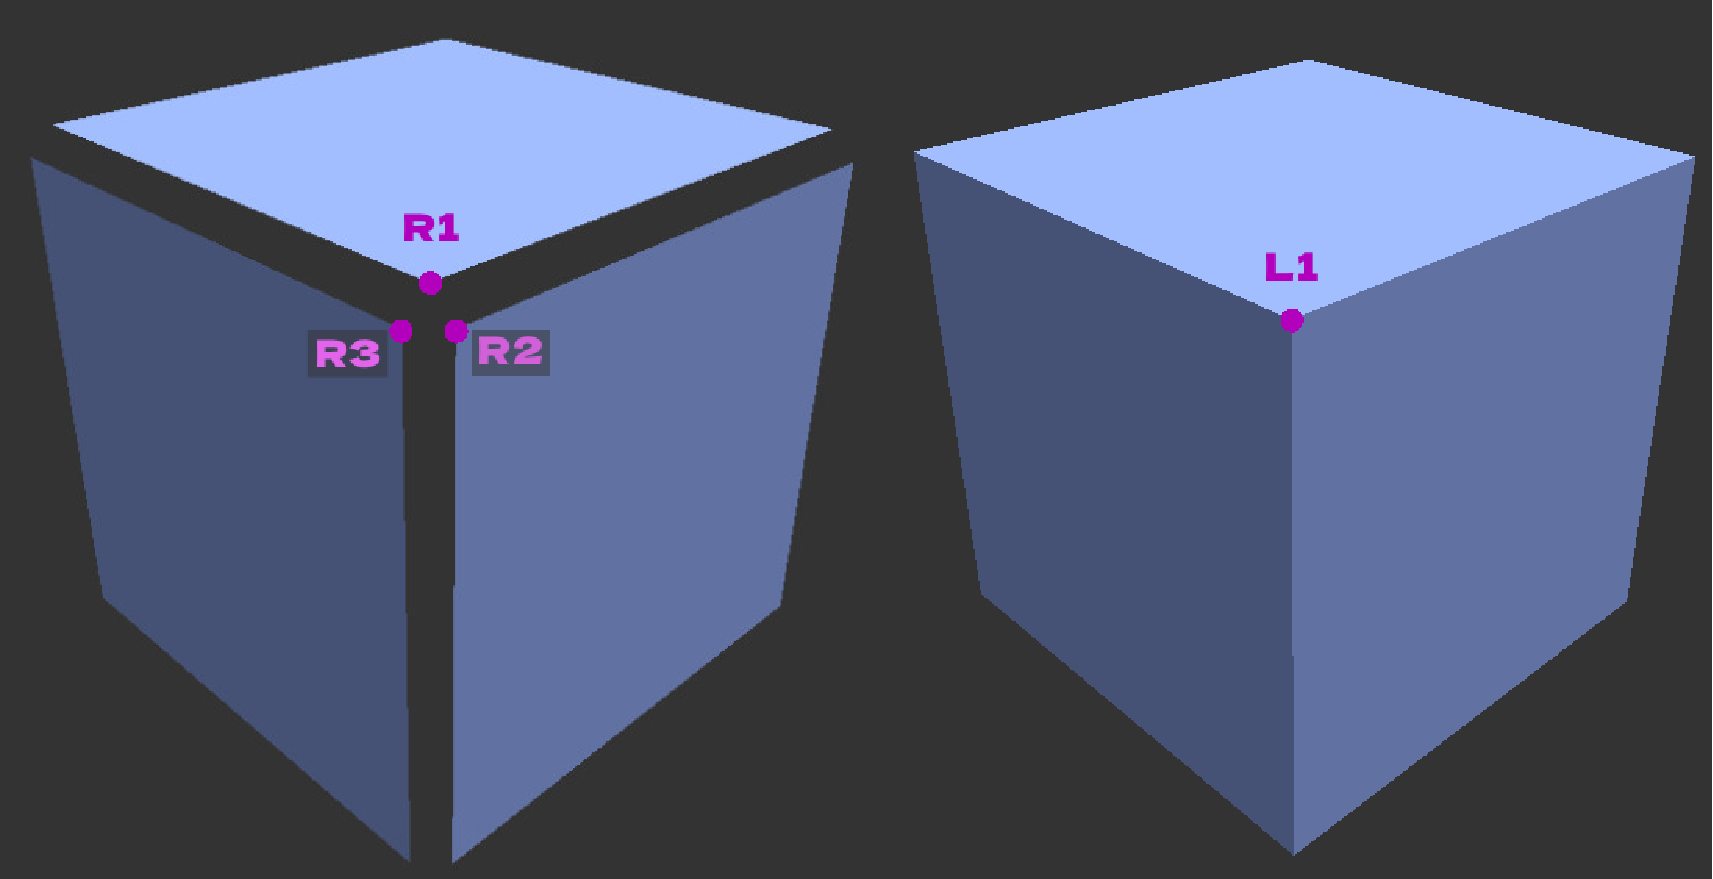
\includegraphics[width = 1.0\textwidth]{TFGTeXiS-UTF8/Imagenes/Vectorial/VerticesRYL.pdf}
    \caption{Tres vértices de renderizado se manipulan con uno lógico.}
    \label{fig:vert-renderizado-vs-logico}
\end{figure}

En lo sucesivo, nos referiremos a los vértices tal como los interpreta OpenGL (los veinticuatro del cubo) como \textit{vértices de renderizado}, y a las posiciones geométricas únicas que agrupan (los ocho del cubo) como \textit{vértices lógicos}.

\subsubsection{Aristas} \label{sec:aristas}

Se considera una arista como un par de vértices conectados, representado mediante el struct \texttt{Edge}, que almacena los índices de renderizado de sus dos vértices. Una vez cargada la malla, se almacenan todas las aristas relevantes en un vector, con el fin de poder operar sobre ellas posteriormente sin necesidad de reconstruirlas a partir de los polígonos en cada acceso. Como nota, el motivo de almacenar los índices de renderizado y no los de su vértice lógico, es el acceso inmediato sin la necesidad de una indirección adicional que supondría acceder a la posición de esta.

Para generarlas, se recorren los pares de vértices adyacentes de cada polígono que conforma el modelo y se añaden ordenadamente. Con el objetivo de evitar duplicar una arista compartida por dos polígonos adyacentes, se comprueba si este ya ha sido añadido a partir del vértice lógico al que pertenece cada vértice de renderizado, y no de su índice de renderizado directo, ya que dos caras distintas pueden compartir arista utilizando vértices de renderizado distintos entre sí (por poseer normales diferentes). Además, cada par de vértices lógicos se ordena numéricamente, colocando el índice de grupo menor en primer lugar, de manera que una arista $V_1-V_2$ y su equivalente $V_2-V_1$ se consideran la misma arista, independientemente del orden en que aparezcan al recorrer los polígonos.

Este proceso de deduplicación tiene un coste de $O(P \log P)$, siendo $P$ el número total de pares de vértices adyacentes recorridos, ya que se emplea un conjunto ordenado (\texttt{std::set}) para comprobar la existencia previa de cada arista. Una mejora a esto podría ser la implementación en su lugar de una tabla de \textit{hash}, reduciendo su coste a $O(P)$ en promedio.

Este proceso tiene lugar tras la carga completa del modelo, de manera que los vértices lógicos de \texttt{vertexToGroup} están completamente construidos, y la generación de polígonos también ha concluido, puesto que las aristas se construyen a partir de la representación interna de los polígonos.

Almacenar las aristas de forma explícita, en lugar de calcularlas a partir de los polígonos cada vez que se necesitan, resulta especialmente relevante para dos operaciones: la selección de aristas, que itera directamente sobre esta lista en cada iteración del bucle principal de la aplicación, y el resaltado visual de las aristas seleccionadas durante la edición.

\subsubsection{Polígonos} \label{sec:poligonos}

Denominamos polígono a la cara lógica de la malla, esto es, la entidad geométrica con la que interactúa el usuario durante la edición. Cada polígono se representa mediante la estructura \texttt{Polygon}, que almacena una lista ordenada de índices a los vértices de renderizado que delimitan su contorno, al igual que con las aristas, con el objetivo de reducir indirecciones en algunas de sus funciones.

Para el renderizado mediante OpenGL, sin embargo, la geometría debe descomponerse en primitivas triangulares, por lo que cada polígono puede representarse mediante uno o varios triángulos. Durante la carga de la malla, \texttt{tinyobjloader} permite configurar si las caras del modelo se cargan ya trianguladas o si se conserva su estructura original. Dado que, a nivel de usuario, la edición de una malla resulta más intuitiva manteniendo las caras completas en lugar de trabajar directamente sobre triángulos individuales, se opta por este segundo modo, conservando la estructura de cada polígono en la representación interna de la malla.

Los polígonos se almacenan en un vector y se identifican mediante su posición dentro de esta estructura, lo que permite acceder directamente al polígono correspondiente durante el proceso de selección.

\subsection{Selección} \label{sec:seleccion}

El objetivo de este módulo es permitir al usuario seleccionar los distintos elementos lógicos que conforman la malla, ya sean vértices, aristas o polígonos, para posteriormente realizar transformaciones sobre ellos.

Para indicar qué tipo de elemento desea seleccionar, se muestran botones en la interfaz, uno para cada tipo de elemento: selección de vértices, aristas y polígonos. El procedimiento general para detectar qué elemento se está seleccionando consiste en la proyección de los vértices tridimensionales sobre la pantalla, para obtener tanto su posición en dos dimensiones como su profundidad respecto a la cámara. Tras ello, en función del modo de selección, se aplica un algoritmo específico para detectar el elemento.

En consecuencia, el programa calcula y almacena la posición bidimensional y la profundidad de cada vértice de la malla en cada iteración del bucle principal de la aplicación, para poder acceder a estos valores rápidamente durante el resto del proceso de selección.

\subsubsection{Selección de vértices}

Existen dos formas principales de determinar cuál es el vértice que el usuario intenta seleccionar: por un lado, se puede realizar \textit{ray casting} \ref{raycasting} y calcular la distancia entre este rayo y los vértices que componen la malla, para elegir aquél cuya proximidad sea mayor. La alternativa consiste en proyectar los vértices del espacio tridimensional sobre la pantalla, donde se puede posteriormente calcular la distancia euclidiana respecto a la posición del ratón con \texttt{glm::distance}.

En este programa se opta por la segunda opción. El motivo de esta elección es el mejor rendimiento obtenido al operar en dos dimensiones frente a tres.

Dicha proyección sobre la pantalla se calcula una única vez por cada iteración del bucle principal de la aplicación, y se reutiliza por igual en los tres modos de selección (vértices, aristas y polígonos), evitando así proyectar la misma geometría por separado para cada uno. Además, la proyección se realiza únicamente sobre los vértices lógicos de la malla y no sobre sus vértices de renderizado: dado que todos los vértices de renderizado de un mismo grupo comparten exactamente la misma posición (sección~\ref{sec:vertices}), basta con proyectar un único representante por grupo (en nuestro caso, el primer vértice de renderizado de cada uno), evitando así proyecciones redundantes. Con ello, el coste de la proyección es de $O(n)$, siendo $n$ el número de vértices de lógicos de la malla.

Un detalle de interés es que, al proyectar los vértices sobre la pantalla, además de su posición en dos dimensiones se almacena la profundidad a la que se encuentran respecto a la cámara. Si tan solo se midiera la distancia mínima del ratón a cada vértice proyectado, los resultados no serían acertados: dos vértices superpuestos en pantalla, pero situados a distinta profundidad en la escena, resultarían indistinguibles para el criterio de selección. Por ello, el vértice candidato se determina combinando ambos valores: se considera mejor candidato aquél cuya distancia sea claramente menor que la del mejor candidato encontrado hasta el momento. Si la diferencia de distancias entre ambos es despreciable (por debajo de un pequeño margen de tolerancia \texttt{distanceEpsilon}), se prioriza en su lugar el de menor profundidad. De esta manera se resuelven correctamente los casos de vértices próximos entre sí en pantalla, seleccionando el que visualmente se encuentre más cerca de la cámara.

\subsubsection{Selección de aristas}

El primer paso consiste en recorrer todas las aristas de la malla y, para cada una, comprobar si sus dos vértices se encuentran dentro del volumen de vista de la cámara. Dicho de otra forma, si son visibles para la cámara. En caso contrario, la arista se descarta. Debe notarse que esto puede resultar en una arista parcialmente visible quedando descartada, en el caso de que solamente uno de sus vértices sea visible.

A continuación se calcula el punto del segmento proyectado en pantalla más cercano al ratón. Para ello se proyecta la posición del ratón sobre la recta que definen los dos vértices de la arista, obteniendo un parámetro $t$ que indica en qué punto del segmento se sitúa dicha proyección: $t = 0$ corresponde al primer vértice y $t = 1$ al segundo. Este parámetro se limita al intervalo $[0, 1]$, de modo que el punto más cercano se calcula respecto al segmento y no a la recta infinita que lo contiene. Con ello se obtiene el punto del segmento más próximo al ratón, y la distancia euclidiana entre ambos (listing~\ref{lst:mejor_candidato_aristas}).

\begin{listing}[htb]
\begin{minted}[breaklines, fontsize=\small]{glsl}
 const ProjectedVertex& pa = ...;
 const ProjectedVertex& pb = ...;

 if (!pa.visible || !pb.visible)
     continue;

 glm::vec2 ab = pb.screenPosition - pa.screenPosition;

 // Calculo de longitud del vector ab(hacerlo asi evita usar raices cuadradas)
 float len = glm::dot(ab, ab);

 // Ingoramos si el segmento es muy pequeño
 if (len < 0.00001f)
     continue;

 // Determinamos la posicion del raton t sobre el segmento, que resulta en valores entre 0(sobre a) y 1(sobre b)
 float t = glm::dot(mouse - pa.screenPosition, ab) / len;
 t = glm::clamp(t, 0.0f, 1.0f); // Mantenemos valor entre 0 y 1

 // Punto del segmento mas cercano al raton
 glm::vec2 closest = pa.screenPosition + t * ab;

 float dist = glm::distance(mouse, closest);
 float depth = pa.depth * (1.0f - t) + pb.depth * t;

 // Determinamos si es el mejor candidato (selectedEdge)
 if (isBetterCandidate(dist, depth, minScreenDistance, minDepth)) {
     selectedEdge = i;
 }
\end{minted}
\caption{Determinación de mejor candidato entre aristas.}
\label{lst:mejor_candidato_aristas}
\end{listing}

Al igual que con los vértices, la selección de la arista depende de la profundidad a la que se encuentran sus vértices respecto a la cámara. Esta profundidad se interpola linealmente a lo largo de la arista utilizando el mismo parámetro $t$ calculado anteriormente, obteniendo así una estimación de la profundidad del punto de contacto entre el ratón y la arista, que se evalúa junto con la distancia al ratón para determinar el mejor candidato.

Finalmente, un detalle adicional es que solo se considera una arista como candidata válida si su distancia al ratón se encuentra por debajo de un umbral mínimo en píxeles, evitando selecciones accidentales de aristas alejadas del cursor.

\subsubsection{Selección de polígonos} \label{sec:seleccion-poligonos}

Para seleccionar polígonos, se comienza recorriendo todos ellos y descartando aquellos que posean algún vértice fuera del volumen de vista de la cámara.

Para los polígonos restantes, se comprueba si el ratón se encuentra dentro de alguno de los triángulos en los que se descompone cada polígono. Esta descomposición se realiza mediante triangulación en abanico (figura~\ref{fig:fan-triangulation}): se fija el primer vértice del polígono como vértice común, y se forman triángulos tomando, de dos en dos, cada par de vértices consecutivos restantes junto con dicho vértice común.

\begin{figure}[htbp]
    \centering
    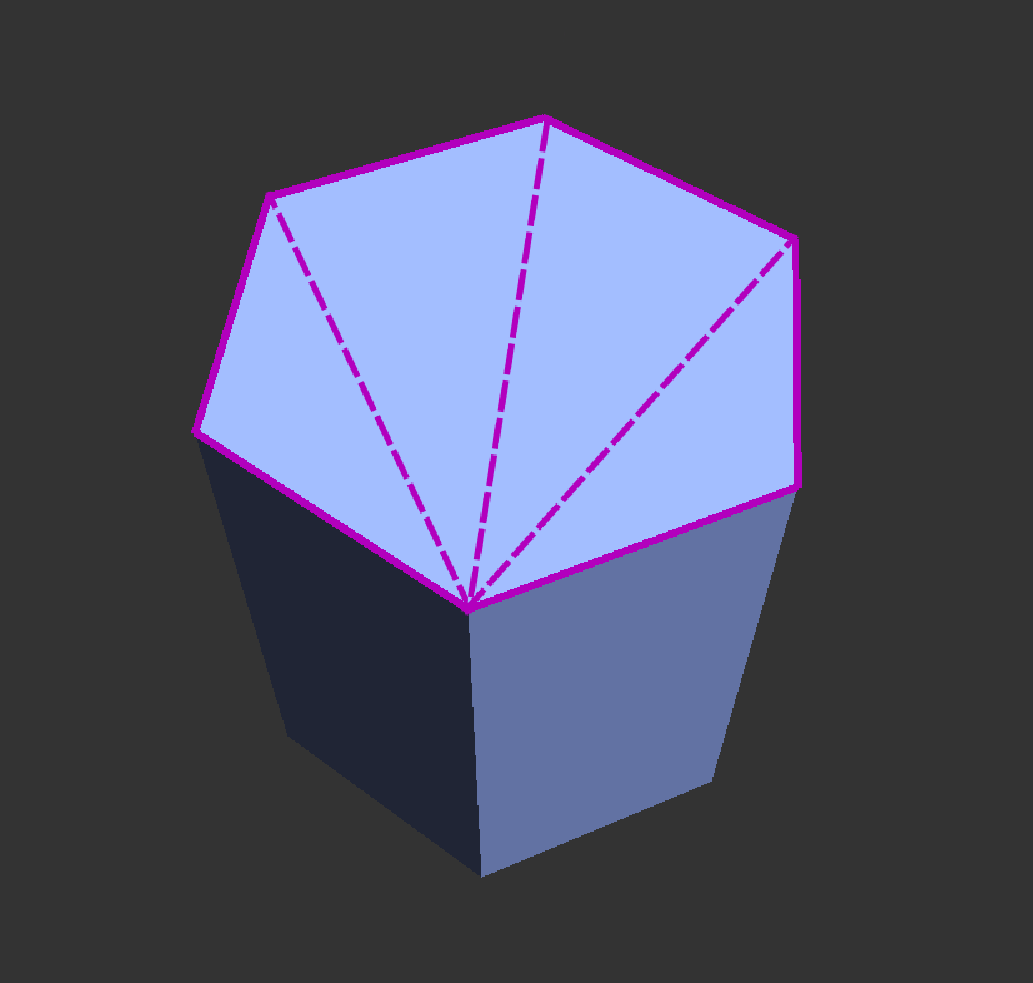
\includegraphics[width = 0.6\textwidth]{TFGTeXiS-UTF8/Imagenes/Vectorial/TriangulacionAbanico.pdf}
    \caption{Triangulación de polígono en abanico.}
    \label{fig:fan-triangulation}
\end{figure}

Para determinar si el ratón se encuentra dentro de cada uno de estos triángulos, se emplea el cálculo de coordenadas baricéntricas (código~\ref{code:point-in-triangle}). Si alguno de los triángulos en los que se divide el polígono contiene la posición del ratón, se calcula la profundidad que tiene respecto a la cámara, y si es el polígono que se encuentra a menor profundidad de entre todos los candidatos, queda marcado como mejor candidato.

\begin{listing}[htb]
\begin{minted}[breaklines, fontsize=\small]{c++}
bool Selector::pointInTriangle(const glm::vec2& p, const glm::vec2& a,
                                const glm::vec2& b, const glm::vec2& c,
                                float& u, float& v) {
    glm::vec2 v0 = c - a;
    glm::vec2 v1 = b - a;
    glm::vec2 v2 = p - a;

    float dot00 = glm::dot(v0, v0);
    float dot01 = glm::dot(v0, v1);
    float dot02 = glm::dot(v0, v2);
    float dot11 = glm::dot(v1, v1);
    float dot12 = glm::dot(v1, v2);

    float invDenom = 1.0f / (dot00 * dot11 - dot01 * dot01);
    u = (dot11 * dot02 - dot01 * dot12) * invDenom;
    v = (dot00 * dot12 - dot01 * dot02) * invDenom;

    return (u >= 0.0f) && (v >= 0.0f) && (u + v <= 1.0f);
}
\end{minted}
\caption{Comprobación de punto dentro de triángulo mediante cálculo de coordenadas baricéntricas.}
\label{code:point-in-triangle}
\end{listing}

\subsection{Cámara} \label{sec:camera}

Manipular un elemento tridimensional requiere que el usuario lo pueda observar desde múltiples ángulos. Con este fin se desarrolla una cámara que ofrece al usuario diversas opciones para manejarla.

Tal como se describe en la sección~\ref{sec:pipeline-coordenadas}, la cámara interviene en el pipeline de renderizado a través de la matriz de vista. Para su funcionamiento, se definen las variables de posición de la cámara, el objetivo hacia el que mira, y la dirección ``arriba'' del mundo (en este caso, el eje $(0, 1, 0)$, por convención general). Estas variables permiten posteriormente realizar las distintas operaciones sobre cómo la cámara observa las mallas del mundo tridimensional. Además, se mantiene una variable para indicar el tipo de proyección que usa la cámara, perspectiva u ortogonal, que también afecta al funcionamiento del zoom, como se describe más adelante.

Con todo esto se desarrollan las tres operaciones principales con las que se puede manipular la cámara:

\textbf{Órbita:} la cámara gira alrededor del objetivo indicado, mediante el uso del botón central del ratón. Para determinar la nueva posición de la cámara se toma el desplazamiento del ratón en pantalla en los ejes $X$ e $Y$, y en función de este se modifican el \emph{pitch} y el \emph{yaw} de la cámara (los ángulos de inclinación vertical y de giro horizontal respecto al objetivo). Para evitar saltos bruscos al alcanzar una orientación paralela al eje vertical, se establecen límites máximos para el valor del \emph{pitch}. A continuación se calcula la nueva dirección de la cámara, que se normaliza, y junto con la posición del objetivo y la distancia a la que se encuentra la cámara de este, se obtiene la nueva posición de la cámara.

\textbf{Paneo:} permite desplazar la vista en el plano actual de la cámara, tanto horizontal como verticalmente. Se usa nuevamente el desplazamiento del cursor en pantalla para determinar cuánto deben desplazarse la cámara y su objetivo, cambiando así el punto alrededor del cual orbita la cámara.

\textbf{Zoom:} varía su funcionamiento en función del tipo de proyección de la cámara. En perspectiva, se incrementa o decrementa la distancia entre la cámara y el objetivo, lo cual sí produce un efecto de acercamiento visual, ya que en este tipo de proyección las líneas de proyección convergen hacia la cámara, y por tanto el tamaño aparente de un objeto en pantalla depende de su distancia a esta. En la proyección ortogonal, en cambio, las líneas de proyección son paralelas entre sí en lugar de converger hacia la cámara, por lo que el tamaño aparente de un objeto no varía con su distancia a la cámara, y acercarla o alejarla no produciría ningún efecto visual de zoom.

Por este motivo, en proyección ortogonal el zoom actúa en su lugar directamente sobre el volumen de vista: la variable \texttt{orthogonalZoom} determina la mitad de la altura de dicho volumen, a partir de la cual se calcula su mitad de anchura aplicando la relación de aspecto de la ventana, y ambos valores se emplean para construir la matriz de proyección ortogonal. Reducir \texttt{orthogonalZoom} estrecha el volumen de vista, haciendo que el modelo ocupe una porción mayor de la pantalla, y aumentarlo produce el efecto contrario.

Un detalle común a las tres operaciones de la cámara es que, antes de aplicarlas, el desplazamiento del ratón se multiplica por la distancia actual de la cámara al objetivo: de esta manera, si la cámara se encuentra ya próxima a este, el movimiento resultante será menor, y viceversa, permitiendo al usuario un control más preciso. La única excepción es el zoom en proyección ortogonal, que modifica \texttt{orthogonalZoom} en una cantidad fija por cada evento de \emph{scroll}, sin multiplicarla por ninguna distancia: al no existir, en este modo, una distancia entre cámara y objetivo que determine el tamaño aparente del modelo (según se ha explicado), no hay ninguna magnitud equivalente por la que escalar el movimiento, y su sensibilidad percibida no varía en función de lo alejada o cercana se encuentre la cámara del objetivo.

Finalmente, se debe tener en cuenta el espacio de recorte de la cámara: una vez obtenida la proyección de vista, se descarta aquello que se encuentre demasiado cerca o demasiado lejos de la cámara. Para ello, la cámara mantiene dos variables de recorte: una que indica la distancia mínima por debajo de la cual un objeto deja de renderizarse por estar demasiado cerca, establecida en 0.1 unidades, y otra para la distancia máxima, establecida en 100 unidades.

\subsection{Operaciones de manipulación}

El proyecto ofrece diversas operaciones realizables sobre el elemento actualmente seleccionado.

\subsubsection{Transformación}

La operación de transformación permite aplicar traslación, rotación o escalado sobre los elementos seleccionados. Se inicia al pulsar el botón del ratón sobre un elemento ya seleccionado, se actualiza en cada iteración del bucle principal mientras dicho botón permanece pulsado, y finaliza al soltarlo.

Al iniciarse, se establece el pivote de la transformación como la media aritmética de las posiciones de los vértices seleccionados, de modo que el resultado de rotar o escalar la selección se perciba centrado en torno a ella. A continuación, se almacenan las posiciones originales de todos los vértices que se verán afectados, y se calcula un plano de arrastre, definido por dicho pivote y la dirección desde la cámara hacia este.

Este plano no interviene por igual en las tres operaciones. En la traslación, se emplea para convertir el movimiento bidimensional del ratón en un desplazamiento tridimensional: en cada iteración se calcula el punto en el que el rayo proyectado desde la posición actual del ratón intersecta con dicho plano, y la diferencia respecto al punto de intersección inicial determina la magnitud de la traslación. La rotación y el escalado, en cambio, se basan directamente en el desplazamiento horizontal del ratón en pantalla, desde la posición en la que se inició la transformación. Únicamente cuando la rotación se realiza sin un eje fijo se reutiliza la normal de este plano, empleándola en ese caso como eje de rotación, orientado de la cámara hacia el pivote, en lugar de como plano de intersección.

En el caso de la rotación, el ángulo se obtiene multiplicando el desplazamiento horizontal por un factor de sensibilidad. En el caso del escalado se sigue un proceso análogo, con la diferencia de que, para un desplazamiento nulo del ratón, el factor de escala debe mantenerse en 1, evitando así que los elementos seleccionados colapsen sobre sí mismos en el instante en que se inicia la transformación.

En los tres casos, la magnitud obtenida se aplica sobre una matriz identidad mediante las funciones correspondientes de \texttt{glm} (\texttt{translate}, \texttt{rotate} o \texttt{scale}), obteniendo así la matriz de transformación resultante. Dicha matriz se aplica a cada vértice seleccionado tomando como referencia su posición original respecto al pivote, y no su posición actual, evitando así una acumulación de error de redondeo si la transformación se actualiza durante muchas iteraciones consecutivas del bucle principal.

Además de mediante arrastre del ratón, la posición de la selección puede ajustarse numéricamente desde un panel de la interfaz (sección~\ref{sec:UI}), que permite fijar directamente cada coordenada del pivote. A diferencia del arrastre, este mecanismo calcula directamente el desplazamiento necesario para que el pivote alcance el valor introducido, y aplica dicho desplazamiento como una traslación. Los dos tipos de transformación permanecen sincronizados, con una modificación del panel de la interfaz transformando el elemento seleccionado, y una alteración de posición de un elemento notificando a la interfaz de la nueva posición del pivote del elemento seleccionado.

Cabe señalar que el cálculo de la transformación se realiza íntegramente en la CPU: se recorren los vértices seleccionados en un bucle, y al finalizar se recalculan las normales de toda la malla y se reenvía el contenido completo del VBO a la GPU, en lugar de únicamente los vértices modificados (sección~\ref{sec:buffers}). Para mallas de gran tamaño, esto implica transferir a la GPU información no modificada en cada iteración del arrastre. Por tanto, una posible mejora sería trasladar el cálculo de la transformación a la propia GPU.

\subsubsection{Eliminación de elementos} \label{sec:eliminacion}

Otra manipulación disponible sobre la malla es la eliminación de elementos, cuyo comportamiento varía según el tipo de elemento seleccionado.

Si la selección actual son polígonos, estos se eliminan directamente de la lista de polígonos de la malla. Si la selección son aristas, para cada arista seleccionada se recorren todos los polígonos de la malla comprobando si alguna de sus aristas coincide con ella. Todo polígono que contenga la arista seleccionada queda marcado para su eliminación. Si la selección son vértices, se eliminan todos los polígonos que hagan uso de alguno de los vértices seleccionados. En los tres casos, el resultado del proceso es siempre el mismo: un conjunto de polígonos marcados para su eliminación, sobre el que se aplica a continuación un procedimiento común.

Dicho procedimiento no elimina explícitamente ninguna arista ni ningún vértice de forma individual. Las aristas, al no almacenarse de forma incremental sino reconstruirse por completo a partir de los polígonos supervivientes (sección~\ref{sec:aristas}), dejan automáticamente de incluir cualquier arista que perteneciera únicamente a los polígonos eliminados, sin necesidad de localizarla y eliminarla de forma independiente. Los vértices, por su parte, pueden quedar sin ningún polígono que los referencie tras eliminar los polígonos marcados; por ello, se recorre la lista de vértices para identificar aquellos que han quedado sueltos, y se eliminan. Dado que esto desplaza los índices de los vértices restantes, se construye una tabla de remapeado que permite actualizar las referencias a vértices en los polígonos supervivientes, así como reconstruir los grupos de vértices lógicos, algunos de los cuales pueden haber desaparecido por completo si todos sus vértices asociados quedaron sueltos. Finalmente, se reconstruye la topología de la malla, lo cual regenera tanto las aristas como los índices de renderizado a partir de los polígonos ya actualizados.

Herramientas de edición de mallas como Blender tienden a ofrecer esta eliminación en cascada, aunque también ofrecen al usuario otras opciones explícitas sobre la geometría que desea conservar \cite{blender-delete}.

\subsubsection{Extrusión} \label{sec:extrusion}

Además de lo anterior, se pueden realizar operaciones de extrusión sobre la malla. Esta operación recibe un único parámetro, la distancia a extruir, y se invoca al pulsar una tecla determinada, aplicándose sobre la selección de polígonos actual con un valor de distancia fijo definido en el propio código. A diferencia de las operaciones de transformación descritas anteriormente, la extrusión no admite en su implementación actual un valor interactivo controlado por el arrastre del ratón.

Para realizarla, se comienza obteniendo la dirección media de las normales de los polígonos seleccionados, ya que esta será la dirección en la que se extruye la selección. A continuación, por cada vértice lógico presente en la selección se crea un nuevo vértice desplazado la distancia indicada en dicha dirección, quedando así diferenciados los vértices nuevos de los originales.

Antes de construir las caras laterales, se determina cuántos de los polígonos seleccionados hacen uso de cada arista. Esto permite distinguir las aristas internas de la selección, compartidas por dos caras seleccionadas adyacentes, de las aristas de borde, pertenecientes a una única cara seleccionada.

Para cada polígono seleccionado se genera un nuevo conjunto de vértices superiores, correspondientes a los vértices desplazados calculados anteriormente. Después, recorriendo cada arista del polígono original, se omite la creación de una cara lateral si dicha arista es interior a la selección. En caso contrario, se construye un nuevo polígono cuadrangular que une los dos vértices originales de la arista con sus correspondientes vértices desplazados, cerrando así el lateral de la extrusión. Finalmente, el polígono original se actualiza para que use directamente los nuevos vértices superiores, pasando a formar la cubierta de la extrusión, y se reconstruye la topología de la malla.

\subsection{Ratón y teclado} \label{sec:input}

La aplicación gestiona el input del usuario a través de dos vías independientes, teniendo en cuenta una peculiaridad del sistema de atajos de teclado de Qt.

Determinadas acciones de la interfaz (el modo de selección, el modo de transformación, el eje activo, el modo de renderizado y el tipo de proyección) se activan mediante teclas registradas como atajos de \texttt{QAction} en \texttt{MainWindow} con \mintinline[breaklines, breakafter=::,fontsize=\small]{c++}{QAction::setShorcut(...)}, cada una conectada directamente a un método del \texttt{Editor}. Qt resuelve estos atajos mediante su propio sistema de gestión de teclado a nivel de aplicación, el cual intercepta el evento correspondiente antes de que este llegue al \textit{widget} de renderizado (\texttt{Canvas}). En consecuencia, ninguna de estas teclas resulta detectable a través del resto del sistema de \textit{input} del programa.

El resto del \textit{input} (resto de teclas del teclado, así como los botones y la rueda del ratón) se captura en los manejadores de eventos de \texttt{Canvas}, que reenvían cada evento a la clase \texttt{Input} a medida que Qt se los entrega. Esta clase se implementa mediante miembros y métodos estáticos, lo que permite consultar su estado desde cualquier punto del programa sin necesidad de una referencia.

Es \texttt{Editor} quien gestiona el comportamiento durante una iteración del bucle principal del programa para \texttt{Input}: al inicio de cada iteración invoca \texttt{Input::update()}, y al final, \texttt{Input::endFrame()}. Es \texttt{Editor} quien consulta, junto con \texttt{Camera}, dicho estado, y así determina el comportamiento del programa en cada iteración.

Para distinguir si una tecla se ha pulsado en el frame actual de si simplemente permanece pulsada, se mantiene una copia del estado del frame anterior (\texttt{previousPressedKeys}), actualizada al final de cada frame. La comparación entre ambos conjuntos permite ofrecer dos consultas distintas: \texttt{isKeyDown}, que indica si una tecla está pulsada en un instante dado, e \texttt{isKeyPressed}, que solo resulta cierta durante el frame exacto en que la tecla pasa a estar pulsada. El mismo mecanismo se aplica a los botones del ratón, permitiendo además detectar mediante \texttt{isMouseButtonUp} el instante en que se suelta un botón, empleado para finalizar una operación de transformación en curso.

El desplazamiento del ratón entre frames se calcula invirtiendo el signo de su componente vertical (código~\ref{code:input-delta}):

\begin{listing}[htb]
\begin{minted}[breaklines, fontsize=\small]{c++}
deltaX = mouseX - lastMouseX;
deltaY = lastMouseY - mouseY;
\end{minted}
\caption{Cálculo del desplazamiento del ratón entre frames.}
\label{code:input-delta}
\end{listing}

Esto compensa que las coordenadas de pantalla de Qt crecen hacia abajo, mientras que un desplazamiento hacia arriba del ratón se espera como positivo en el resto del programa. Resolver esta inversión una única vez evita tener que repetirla en cada usuario del desplazamiento del ratón, como la órbita o el paneo de la cámara (sección~\ref{sec:camera}).

Por último, a diferencia del resto del estado de input, el desplazamiento acumulado de la rueda del ratón se reinicia al final de cada frame, ya que solo tiene sentido como una medida de cuánto se ha desplazado la rueda durante ese frame concreto: de no reiniciarse, el último valor de desplazamiento registrado seguiría aplicándose de forma indefinida en frames posteriores en los que el usuario ya no interactúa con la rueda.